% !TeX document-id = {a39e8ab2-a52f-4b84-8569-c61394829c2b}
% !TeX TXS-program:compile = txs:///lualatex/[--shell-escape]
% !TeX TXS-program:lualatex = lualatex -synctex=1 -interaction=nonstopmode --shell-escape %.tex
\documentclass[english, a4paper]{article}

\usepackage[english]{babel}
\usepackage{inputenc}
\usepackage{xcolor}
%\usepackage[usenames, dvipsnames]{color}
\definecolor{mygray}{RGB}{198,198,198}

\usepackage{listings}
\usepackage{minted}
\setminted{breaklines, linenos, bgcolor=mygray, tabsize = 3}

\usepackage{amsthm}
\usepackage{amsmath}
%For danish setup
\usepackage{babel}

\usepackage[T1]{fontenc}
\usepackage{siunitx}				% Enheder i math mode
\usepackage[hidelinks]{hyperref} % clickable refs
\usepackage[backend=biber,style=alphabetic,hyperref]{biblatex} % Needed for bibliography
\usepackage{graphicx}
\usepackage{tabularx}

\usepackage{longtable}
\usepackage{tabu}

\usepackage{cleveref}
\usepackage{subcaption}




\bibliography{references} % Needed for bibliography
\graphicspath{{graphics/}}



\title{E3DSB Miniprojekt A} 
\author{	Simon Alexander Alsing, 201304202\\
			Lasse Østerberg Sangild, 20114274\\
			Tobias Kalhøj, 201505974}
\begin{document}

\maketitle

\newpage
\tableofcontents
\newpage

% !TEX root = main.tex

\section{Introduction}
This project investigates the usage of different digital filters as equalizers. The filter types used are Finite Impulse Respones (FIR) and Infinite Impulse Response (IIR) filters.

FIR filters has a finite memory, and only allows an impulse response to affect the system for a FINITE amount of time.
IIR filters allows the impulse response to affect the system for an INFINITE amount of time.
There are a few key differences between the FIR and IIR.
A FIR filter can run on integer math, whereas IIR requires floating point for the calculations not to blow up. The phase is kept much more stable by using a FIR filter, compared to an IIR filter.
An IIR filter requires fewer coefficients, less memory and is generally faster than a FIR filter.

For this project we are asked to divide the filters into five different bands. Generelly speaking the human hearing is between \SI{20}{\hertz} and \SI{20}{\kilo\hertz} The five bands are taken from \href{https://en.wikipedia.org/wiki/Audio\_frequency}{here} and are adjusted to fit our range of five bands in the range of \SIrange{20}{20000}{\hertz} and are seen in \cref{tab:FiveBand}.

\begin{table}[h]
	\caption{The frequency bands filtered out.}
	\label{tab:FiveBand}
	\begin{tabularx}{\textwidth}{X X}
		\textbf{Frequency} (\si{\hertz})	& \textbf{Description} \\
		\toprule
		\numrange{0}{32}		& The lower human threshold. \\
		\numrange{32}{512}		& Rythm frequencies. \\
		\numrange{512}{2048}	& Horn like and tinny quality. Regular speach lies here. \\
		\numrange{2048}{8192}	& Labial and fricative sounds. \\
		\numrange{8192}{20000}	& Sounds of bells and ringing. \\
	\end{tabularx}
\end{table}

Lav i Matlab en audio equalizer. Equalizeren skal kunne justere niveauet på et indkommende lydsignal individuelt i fem forskellige frekvensbånd fordelt over (og dækkende) det hørbare spektrum med +/- 12 dB. Eksempelvis et bånd fra 0 hertz (eller måske 20 Hz) til 200 Hz. Herefter evt. 200-700 Hz og så fremdeles.

Der skal i opgaven indgå filtre af begge typer (FIR og IIR). Man har frie hænder til valg af designmetode. Vinduesmetoden er fin, hvis det skal foregå manuelt, - ellers er fir1.m og butter.m i Matlab gode bud.

Eksperimenter i opgaven med filterorden og knækfrekvenser. Dokumenter eksperimenterne. Equalizerens samlede impulsrespons og overføringskarakteristik (altså amplitude og fase i frekvens-domænet) skal kunne vises. Dvs. den samlede virkning af de fem filtre fra input til output.

\section{Expectations}
\label{sec:expectations}
We are going to do a few experiments comparing FIR and IIR, but also a few investigating the way either of them works.

\begin{table}
	\caption{Comparing equivalent IIR- and FIR filters.}
	\label{tab:IIRvsFIR}
	\begin{tabularx}{\textwidth}{X X X}
		Statement to test	& Expected Result	& Result \\
		\toprule
		The phase is more stable for a FIR filter & The phase of a signal is affected less by running it thorugh a FIR filter than through an IIR filter. & \\
		IIR is faster		& Using tic toc in Matlab during the filtering, IIR filter will yield a lower value. & \\
	\end{tabularx}
\end{table}

\begin{table}
	\caption{Investigation of altering the IIR coefficients.}
	\label{tab:IIRtest}
	\begin{tabularx}{\textwidth}{X X X}
		Statement to test	& Expected Result	& Result \\
		\toprule
		IIR calculation time scales exponentially with increasing coefficients. & By multiplying the coefficients by 2, 4 or 8, the calculation time increases exponentially. & \\
	\end{tabularx}
\end{table}
\clearpage
\section{Using build-in Matlab functions}
\label{sec:functions}
Before digging into the implementation of the analysis, a quick introduction to the functions from matlab that are in use.
\begin{longtabu}{>{\em}X l X}
\normalfont{\textbf{Function}} & Output & \textbf{Description} \\
\hline
audioread(filename) & [y, Fs] & Read an audiofile and put the contents into two outputs. "y" is the sample data, while "Fs" is the sample rate for the data. \\
fft(y) & Y & Computes the discrete Fourier transform (DFT) of y, using a fast Fourier transform algorithm. \\
length(x) & L & Return the length of the largest array dimension in x.  \\
figure(n) & none & Set a new figure for eg a plot to be saved inside. "n" is the figurenumber \\
plot(x, y, c) & none & Plot a x-sequence "x", y-sequence "y" and a color/representation parameter "c". \\
title(titleName) & none & Sets the title of a figure. \\
xlabel(labelName) & none & Sets the label for the x-axis. \\
ylabel(labelName) & none & Sets the label for the y-axis. \\
hold on/off & none & Holds a plot inside a figure when "on" is set, stops the holding of the plot when hold off is set. A new plot after a hold off creates a new figure. \\
grid on & none & set a grid for the plot. \\
max(x) & M & Return the largest elements in an array. \\
mean(x) & m & Return the avarage or mean value of an array. \\
smooth(x, [span], [method]) & xx & Smoothing the data with a default span value of "5" and a default method of "moving". Setting the span and method is optional.\\
semilogx(Y) & h & Plot data on logarithmic scale on the x-axis. \\
legend(label1, ..., labelN, 'Location', 'Value') & none & Creates a box for description of one or more plots, color seperated. The value of Location can be described with nord, west, south, east - or in combination. In the following section the parameter "southwest" is used. \\
cat(dimension, Array1, ..., ArrayN) & C & Concatenate arrays along a specific dimension.  \\
hamming(L) & w & return a L-point symmetric Hamming window in the column vector w. The formula $w(n)$ is described in \cref{sec:windowing}. \\
sum(A) & S & Return the sum of an array, can optionally take another parameter which handle the dimension of the array. \\
saveas(fig, filename, fileformat) & none & Saves a file with a figure "fig", the filename "filename" and the fileformat "fileformat", at the location of the file being executed. \\
xlim([xmin, xmax]) & none & Sets the start and end value on the x-axis of a figure. \\
\end{longtabu}

\clearpage
\section{Frequency analysis}
\label{sec:analysis}

In this following section an analysis will be made of the sound made by a car motor (figure \ref{fig:car}), windmill (figure \ref{fig:windmill}), EKG (figure \ref{fig:ekg}), breaking wine glass (figure \ref{fig:glassBreaking}) and four different genres of music. 
The approach of this analysis will be to plot the signal in the time domain, the fourier transformed signal and then som applied functions described in section \ref{sec:theory}.


\subsection{Car engine}

The original signal from the car engine is seen in figure \ref{fig:car_time}, while the Fourier transformed signal is seen in figure \ref{fig:car_freq}. The following are also Fourier transformed, but have applied smoothing (figure \ref{fig:car_smooth}), zeropadding (figure \ref{fig:car_zero}) and hamming (figure \ref{fig:car_window}). Notice the magnitude difference from the Fourier transformed to the smoothing.

\begin{figure}[htb!]
	\centering
	\subcaptionbox{Time Domain.\label{fig:car_time}}
	{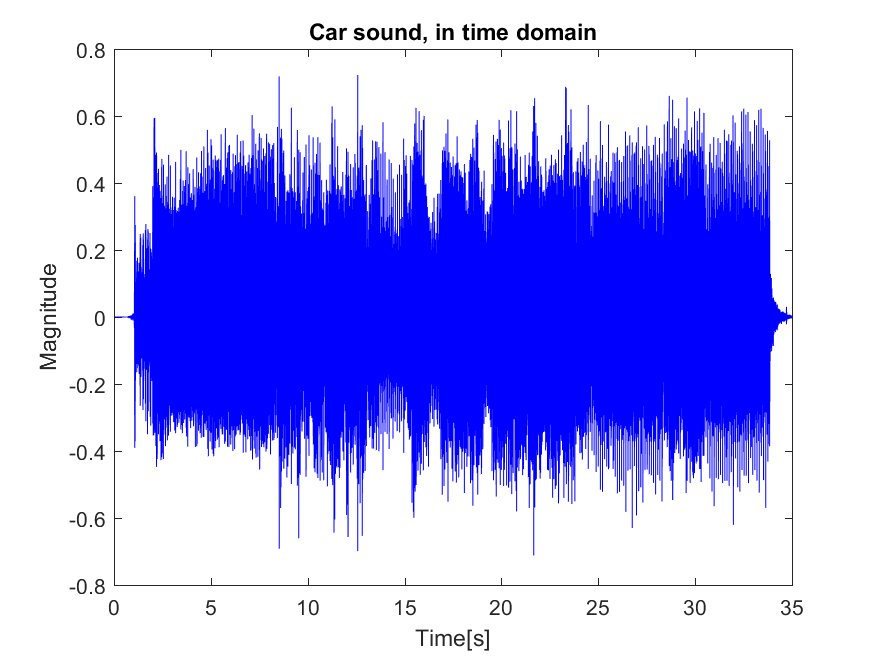
\includegraphics[width=0.45\linewidth]{code/Car_figure1.png}}
	\subcaptionbox{Frequency Domain.\label{fig:car_freq}}
	{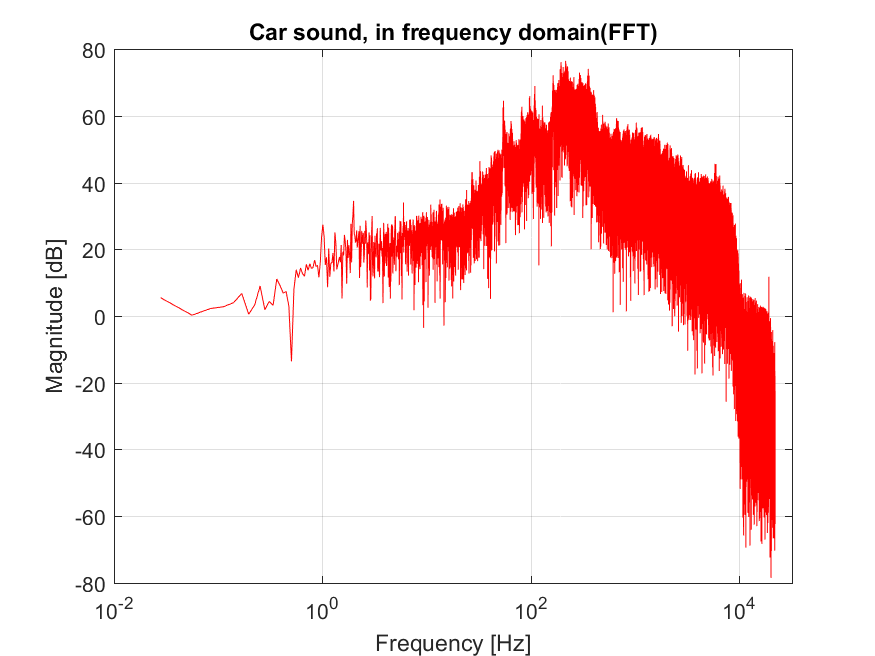
\includegraphics[width=0.45\linewidth]{code/Car_figure2.png}}
	\subcaptionbox{Smoothed fft.\label{fig:car_smooth}}
	{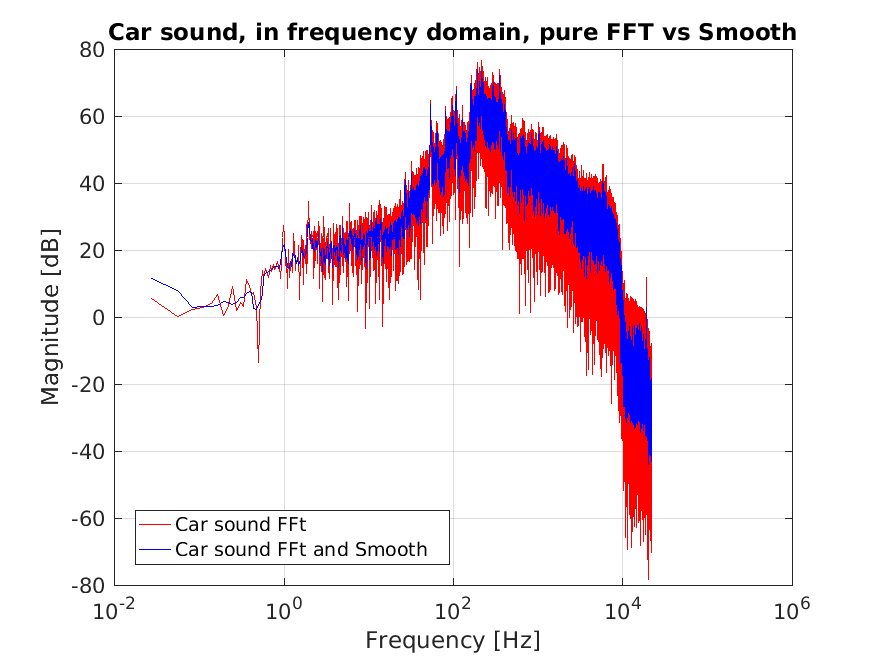
\includegraphics[width=0.45\linewidth]{code/Car_figure3.png}}
	\subcaptionbox{fft of zero padded original.\label{fig:car_zero}}
	{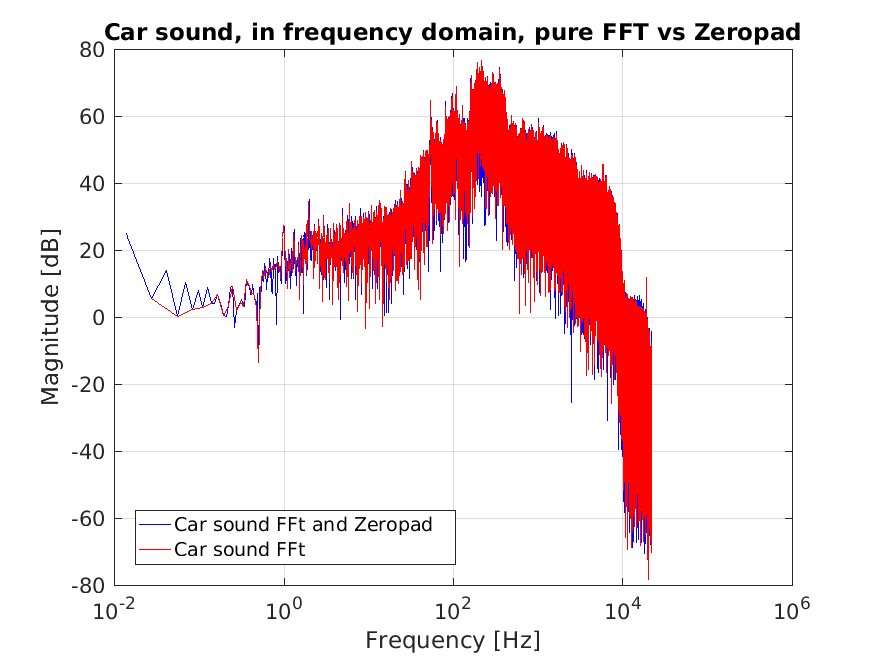
\includegraphics[width=0.45\linewidth]{code/Car_figure4.png}}
	\subcaptionbox{fft of windowed original.\label{fig:car_window}}
	{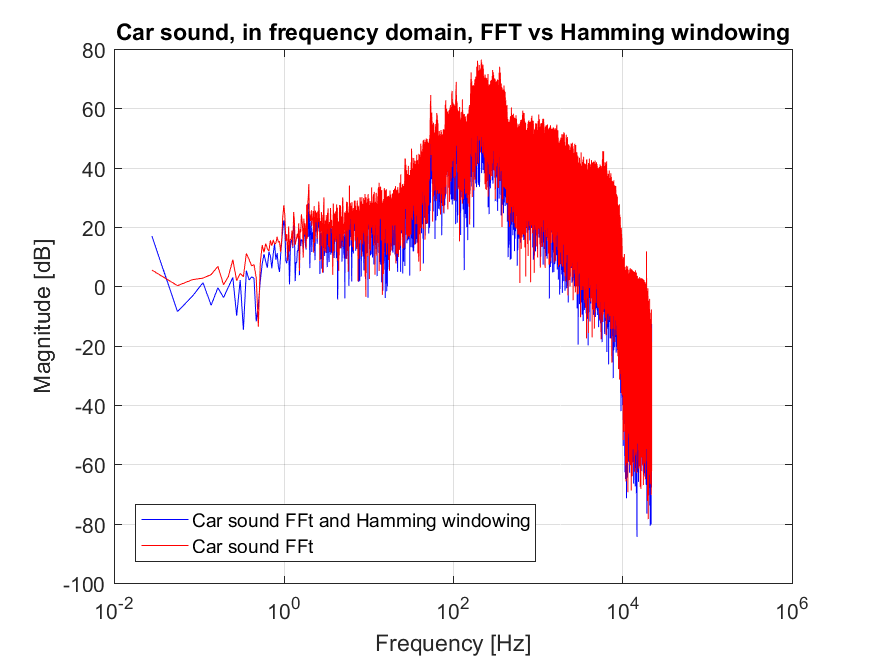
\includegraphics[width=0.45\linewidth]{code/Car_figure5.png}}
	\caption{Analysis of the sound of a car.}\label{fig:car}
\end{figure}
\clearpage

\subsection{Noise from a Windmill}

The original signal from the windmill is seen plotted in the timedomain in figure \ref{fig:windmill_time}, while the fourier transformed signal is seen in figure \ref{fig:windmill_freq}. The following has first applied some function and then is fourier transformed, the smooth function is seen on figure \ref{fig:windmill_smooth}, the zeropadding is seen in figure \ref{fig:windmill_zero} and the window function is seen in figure \ref{fig:windmill_window}.

\begin{figure}[htb!]
	\centering
	\subcaptionbox{Time Domain.\label{fig:windmill_time}}
	{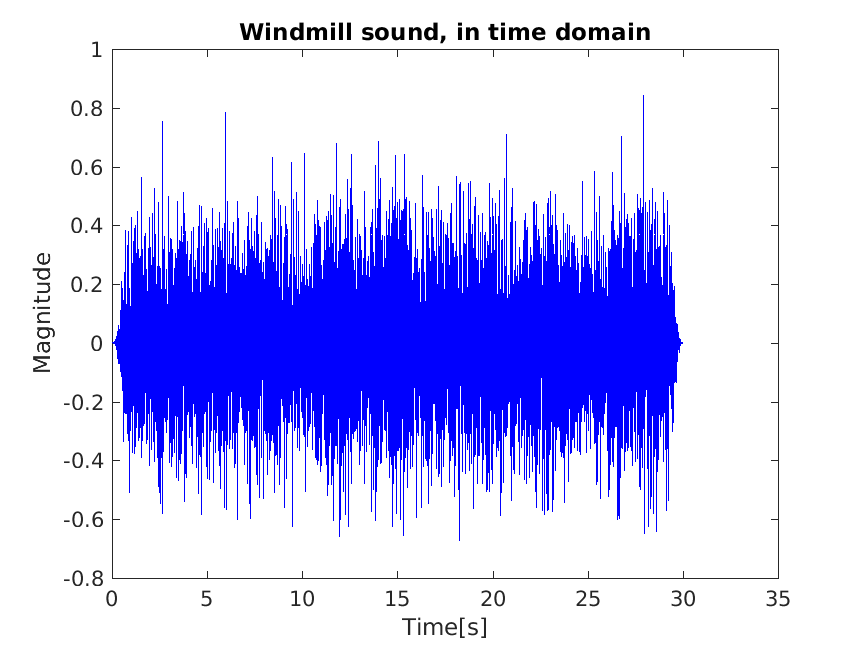
\includegraphics[width=0.45\linewidth]{code/Windmill_figure1.png}}
	\subcaptionbox{Frequency Domain.\label{fig:windmill_freq}}
	{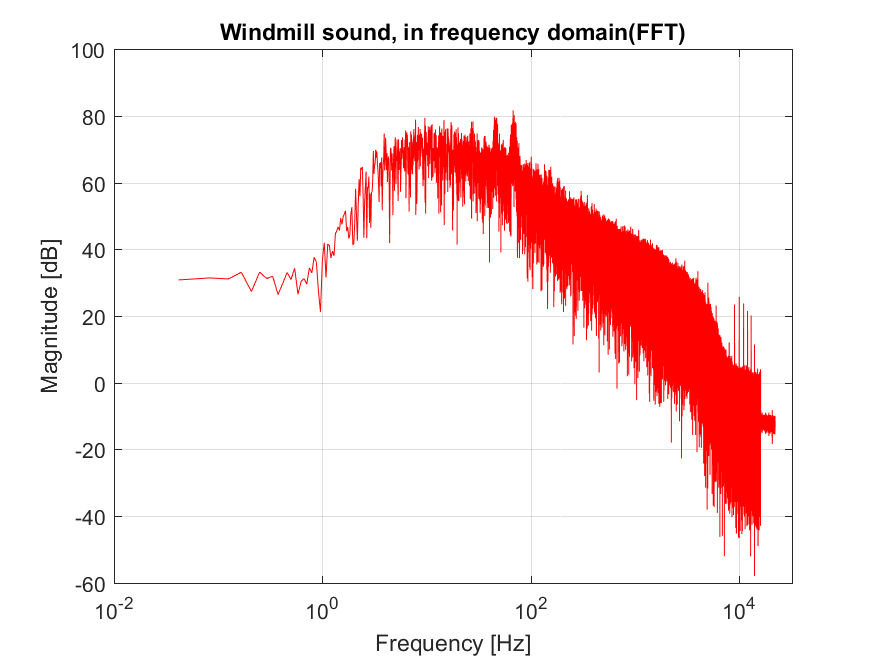
\includegraphics[width=0.45\linewidth]{code/Windmill_figure2.png}}
	\subcaptionbox{Smoothed fft.\label{fig:windmill_smooth}}
	{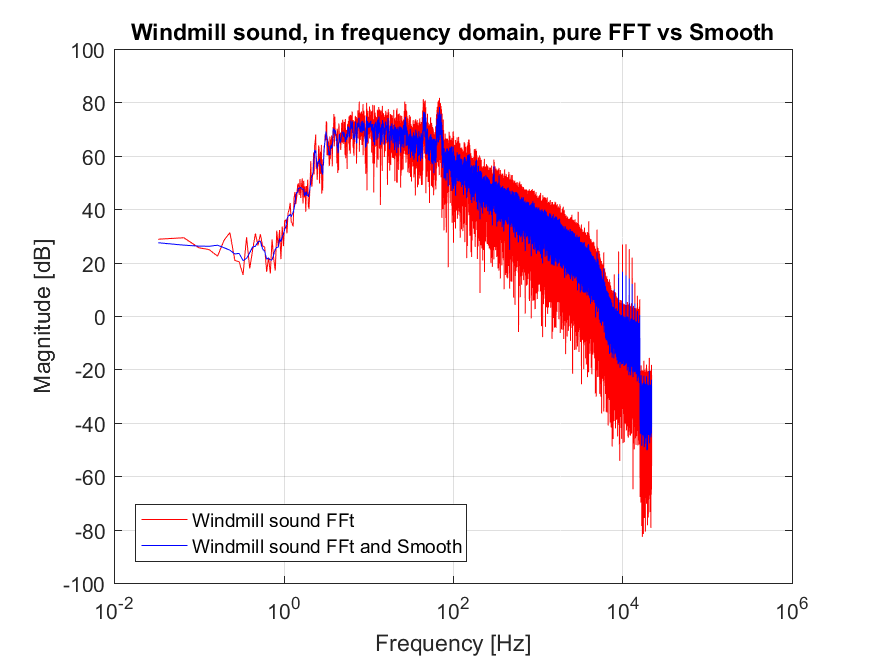
\includegraphics[width=0.45\linewidth]{code/Windmill_figure3.png}}
	\subcaptionbox{fft of zero padded original.\label{fig:windmill_zero}}
	{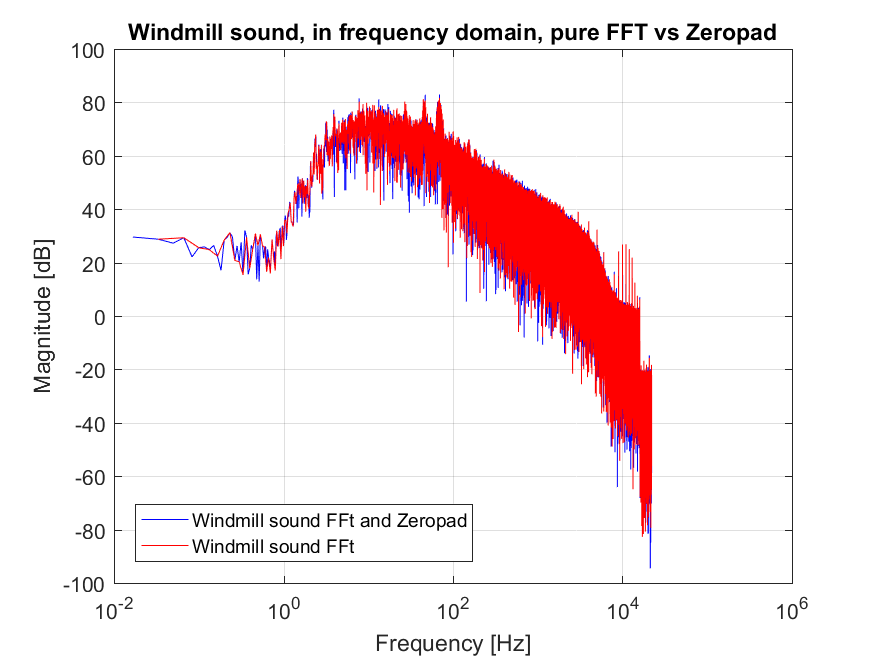
\includegraphics[width=0.45\linewidth]{code/Windmill_figure4.png}}
	\subcaptionbox{fft of windowed original.\label{fig:windmill_window}}
	{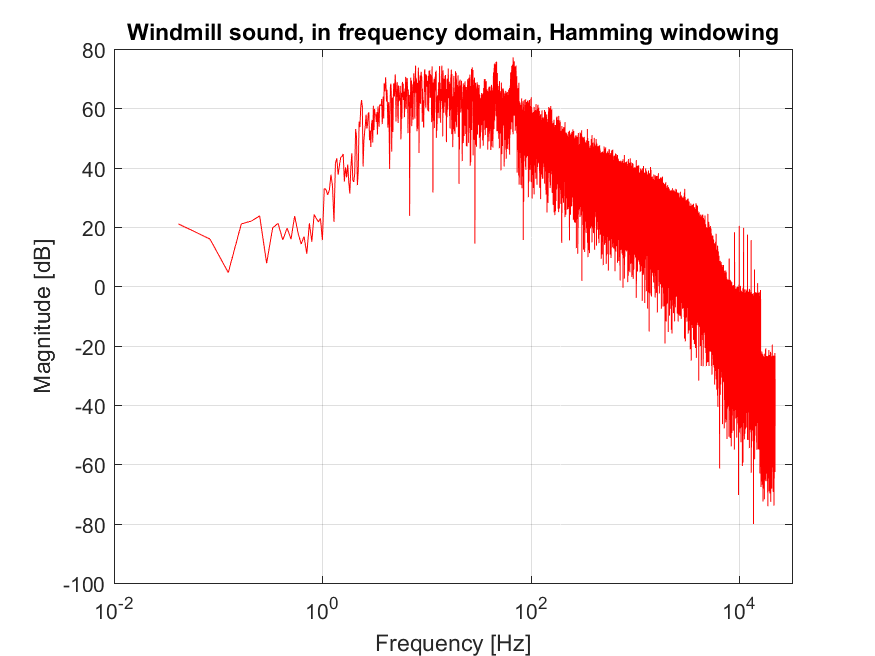
\includegraphics[width=0.45\linewidth]{code/Windmill_figure5.png}}
	\caption{Analysis of the sound of a windmill.}\label{fig:windmill}
\end{figure}


\subsection{EKG}

The original signal from the EKG is seen plotted in the timedomain in figure \ref{fig:ekg_time}, while the fourier transformed signal is seen in figure \ref{fig:ekg_freq}. The following has first applied some function and then is fourier transformed, the smooth function is seen on figure \ref{fig:ekg_smooth}, the zeropadding is seen in figure \ref{fig:ekg_zero} and the window function is seen in figure \ref{fig:ekg_window}.


\begin{figure}[htb!]
	\centering
	\subcaptionbox{Time Domain.\label{fig:ekg_time}}
	{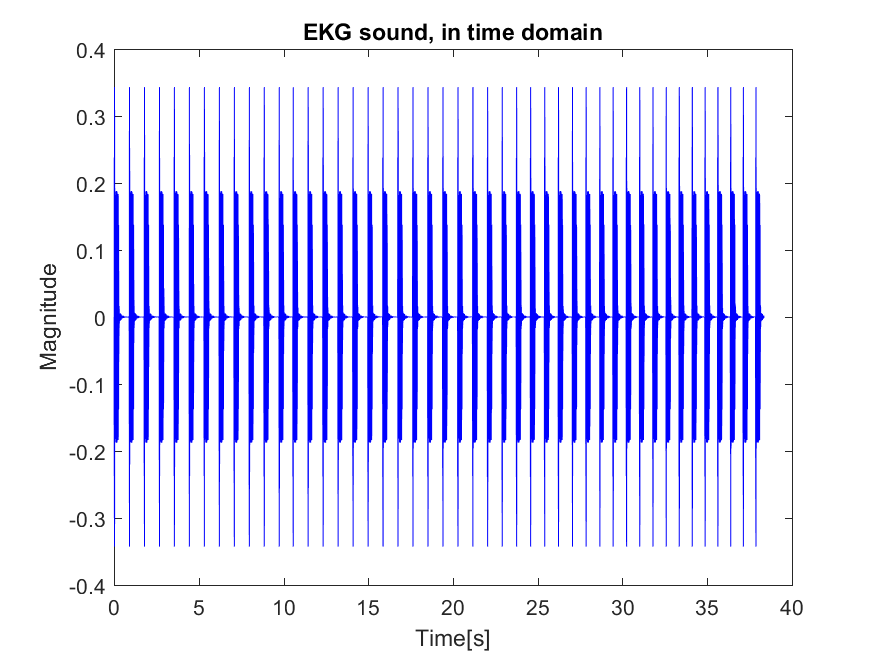
\includegraphics[width=0.45\linewidth]{code/ekg_figure1.png}}
	\subcaptionbox{Frequency Domain.\label{fig:ekg_freq}}
	{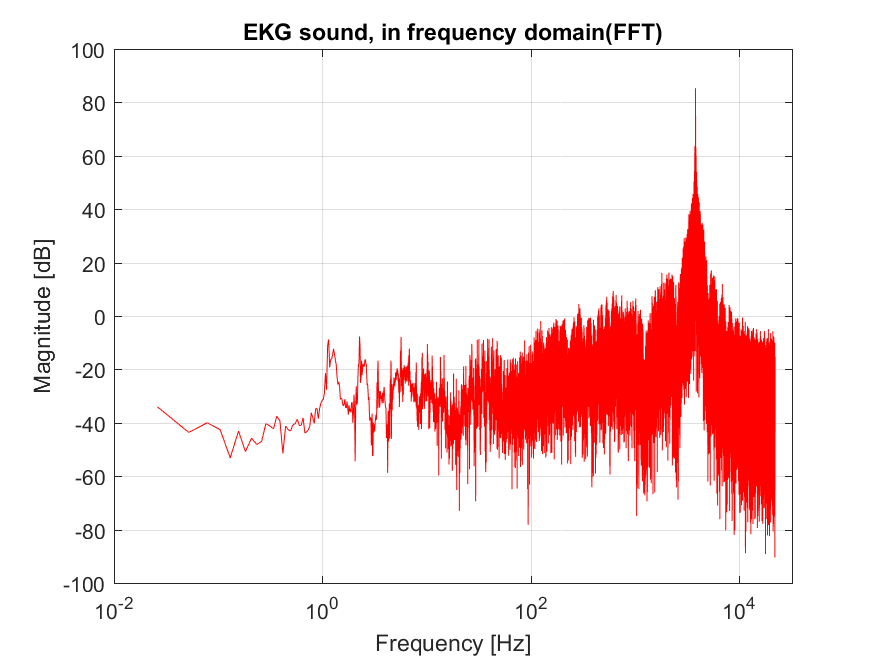
\includegraphics[width=0.45\linewidth]{code/ekg_figure2.png}}
	\subcaptionbox{Smoothed fft.\label{fig:ekg_smooth}}
	{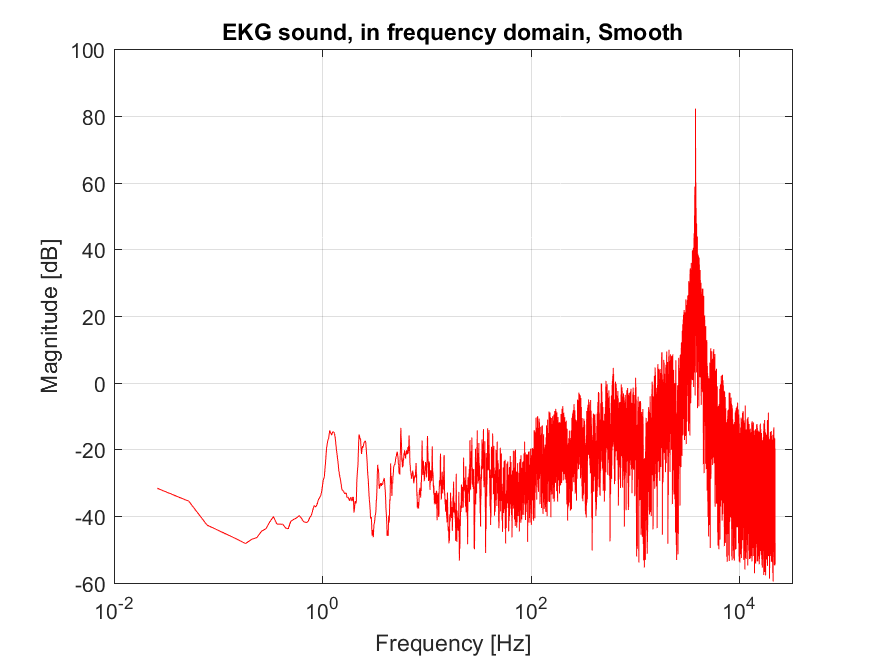
\includegraphics[width=0.45\linewidth]{code/ekg_figure3.png}}
	\subcaptionbox{fft of zero padded original.\label{fig:ekg_zero}}
	{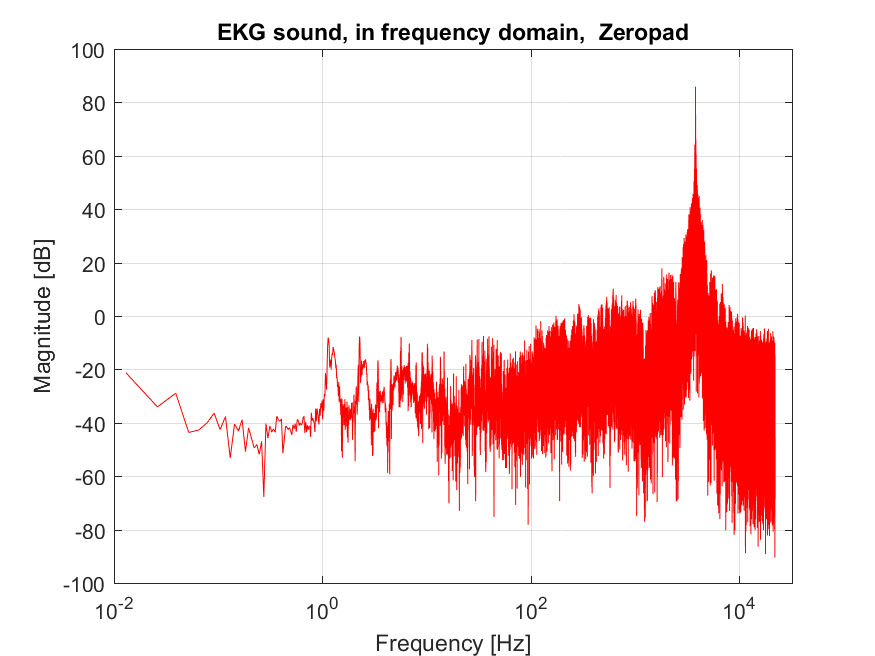
\includegraphics[width=0.45\linewidth]{code/ekg_figure4.png}}
	\subcaptionbox{fft of windowed original.\label{fig:ekg_window}}
	{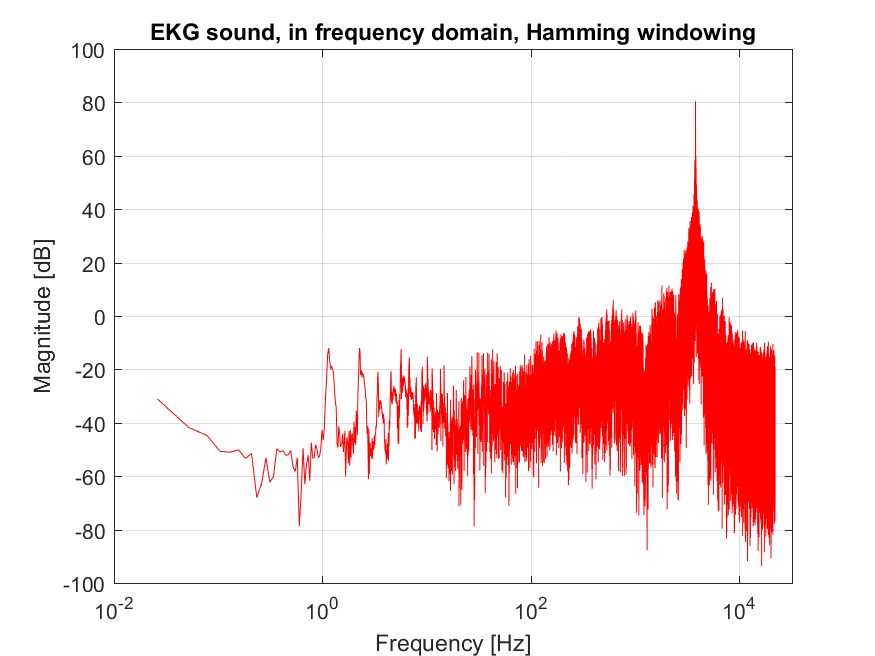
\includegraphics[width=0.45\linewidth]{code/ekg_figure5.png}}
	\caption{Analysis of the sound of an EKG.}\label{fig:ekg}
\end{figure}

\subsection{Breaking Wine Glass}

The original signal from the breaking glass is seen plotted in the timedomain in figure \ref{fig:glassBreaking_time}, while the fourier transformed signal is seen in figure \ref{fig:glassBreaking_freq}. The following has first applied some function and then is fourier transformed, the smooth function is seen on figure \ref{fig:glassBreaking_smooth}, the zeropadding is seen in figure \ref{fig:glassBreaking_zero} and the window function is seen in figure \ref{fig:glassBreaking_window}.

\begin{figure}[htb!]
	\centering
	\subcaptionbox{Time Domain.\label{fig:glassBreaking_time}}
	{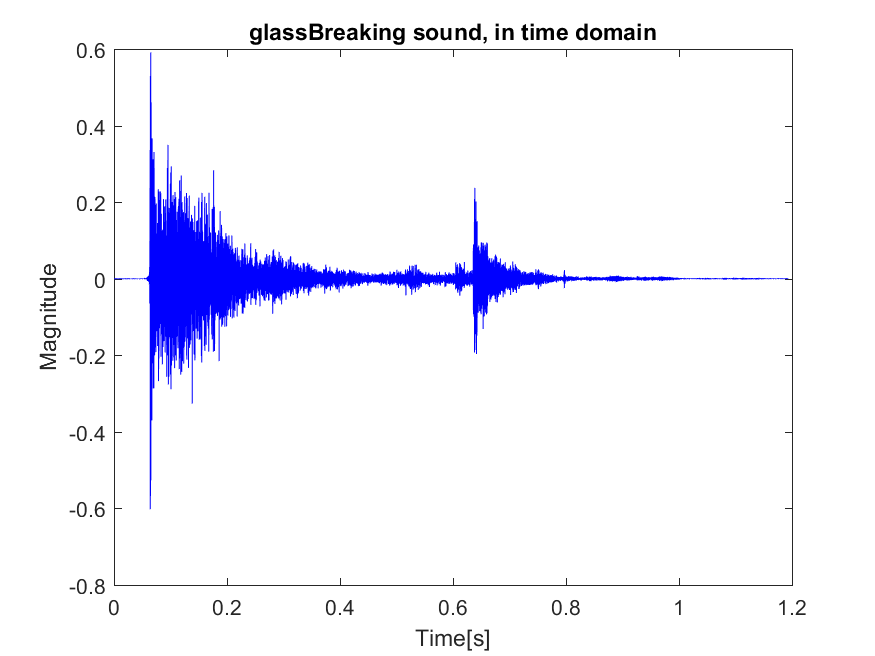
\includegraphics[width=0.45\linewidth]{code/glassBreaking_figure1.png}}
	\subcaptionbox{Frequency Domain.\label{fig:glassBreaking_freq}}
	{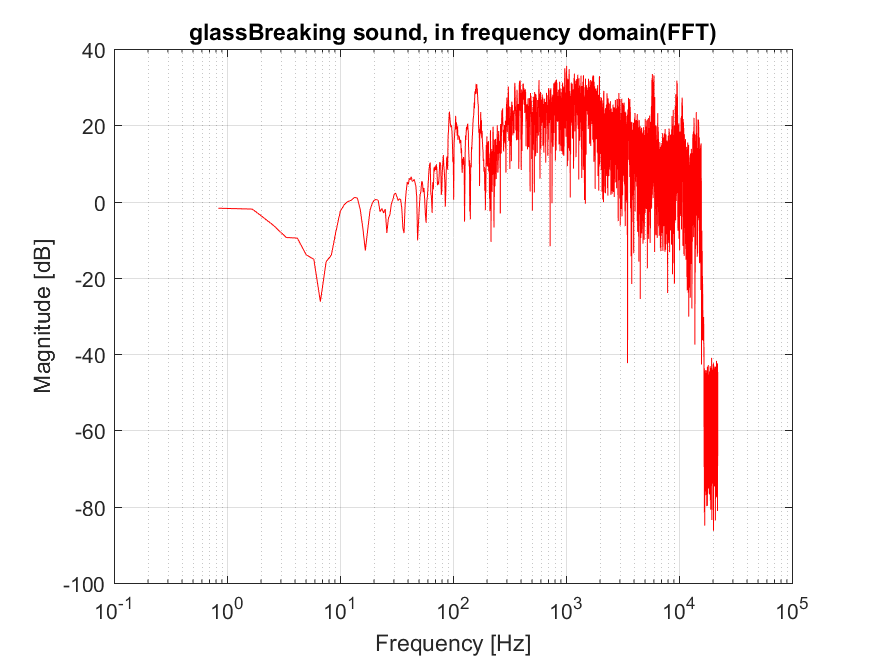
\includegraphics[width=0.45\linewidth]{code/glassBreaking_figure2.png}}
	\subcaptionbox{Smoothed fft.\label{fig:glassBreaking_smooth}}
	{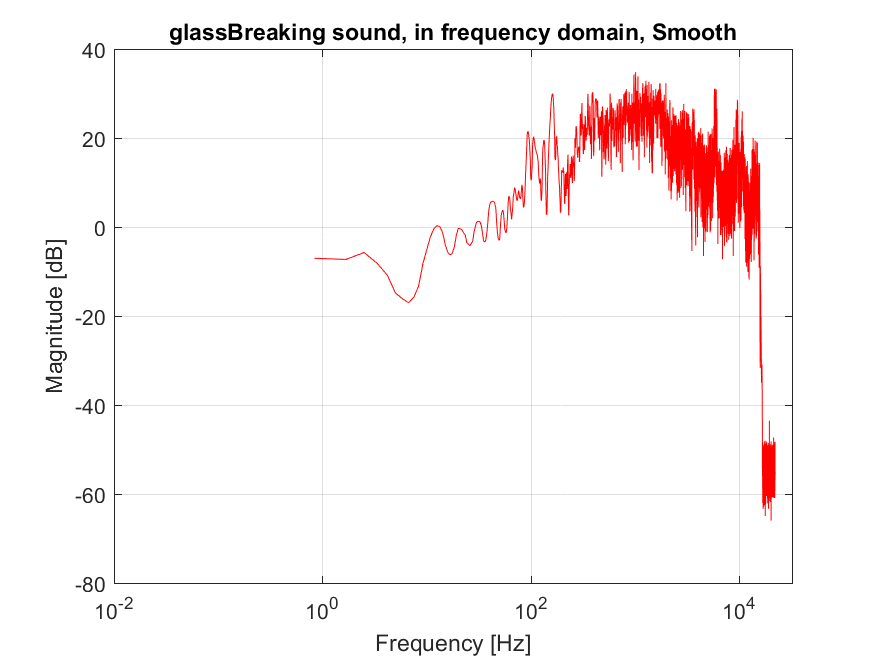
\includegraphics[width=0.45\linewidth]{code/glassBreaking_figure3.png}}
	\subcaptionbox{fft of zero padded original.\label{fig:glassBreaking_zero}}
	{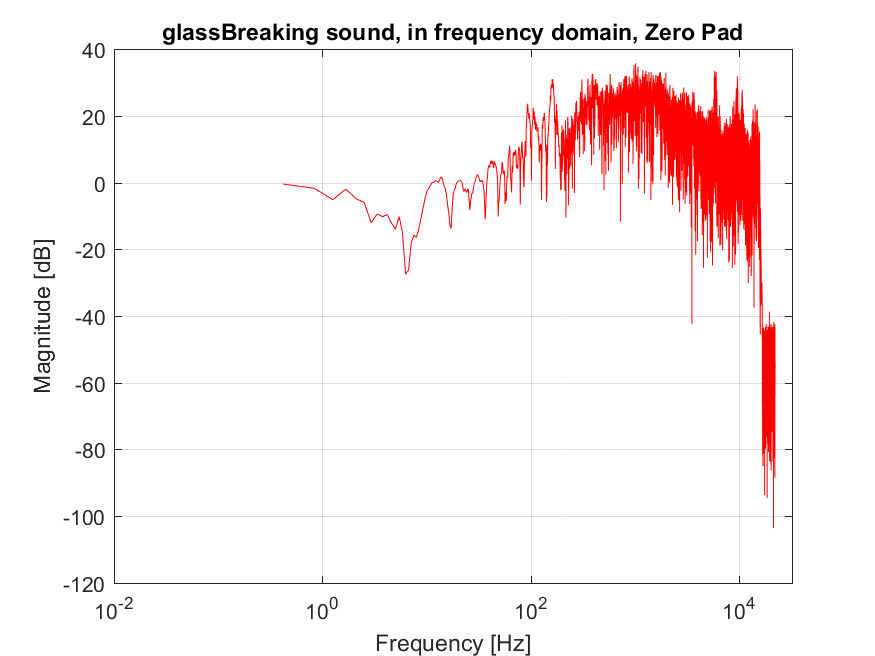
\includegraphics[width=0.45\linewidth]{code/glassBreaking_figure4.png}}
	\subcaptionbox{fft of windowed original.\label{fig:glassBreaking_window}}
	{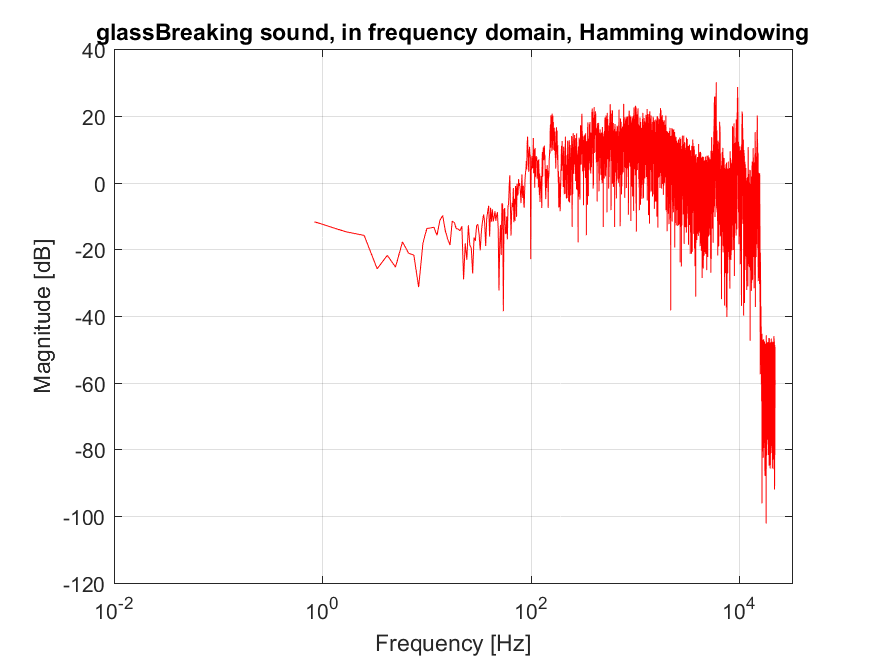
\includegraphics[width=0.45\linewidth]{code/glassBreaking_figure5.png}}
	\caption{Analysis of the sound of a glas breaking.}\label{fig:glassBreaking}
\end{figure}


\subsection{Music}

\paragraph{Pop}
Michael Jackson - Thriller

The original signal from the song "Thriller" is seen plotted in the timedomain in figure \ref{fig:pop_time}, while the fourier transformed signal is seen in figure \ref{fig:pop_freq}. The following has first applied some function and then is fourier transformed, the smooth function is seen on figure \ref{fig:pop_smooth}, the zeropadding is seen in figure \ref{fig:pop_zero} and the window function is seen in figure \ref{fig:pop_window}.


\begin{figure}[htb!]
	\centering
	\subcaptionbox{Time Domain.\label{fig:pop_time}}
	{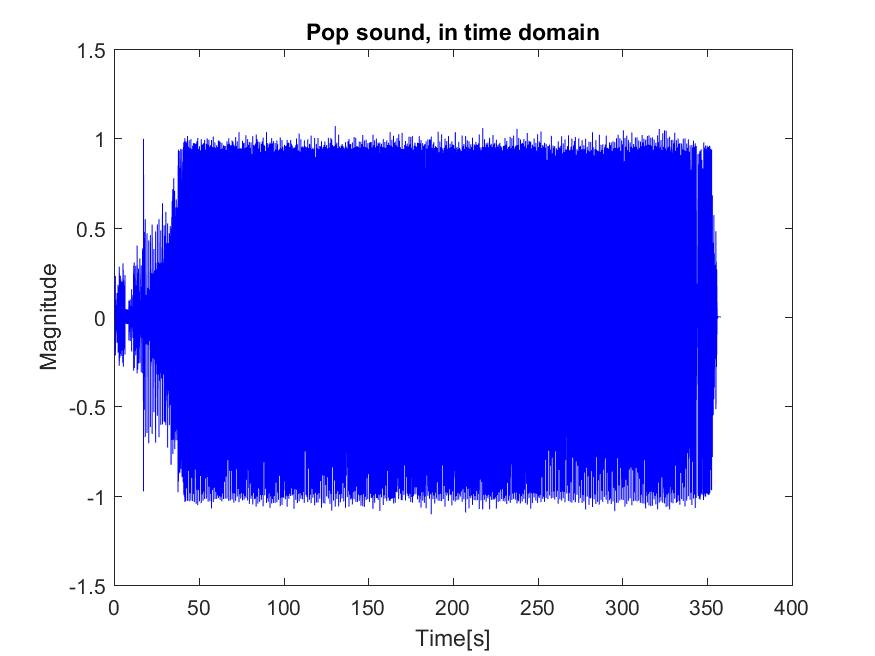
\includegraphics[width=0.45\linewidth]{code/Pop_figure1.png}}
	\subcaptionbox{Frequency Domain.\label{fig:pop_freq}}
	{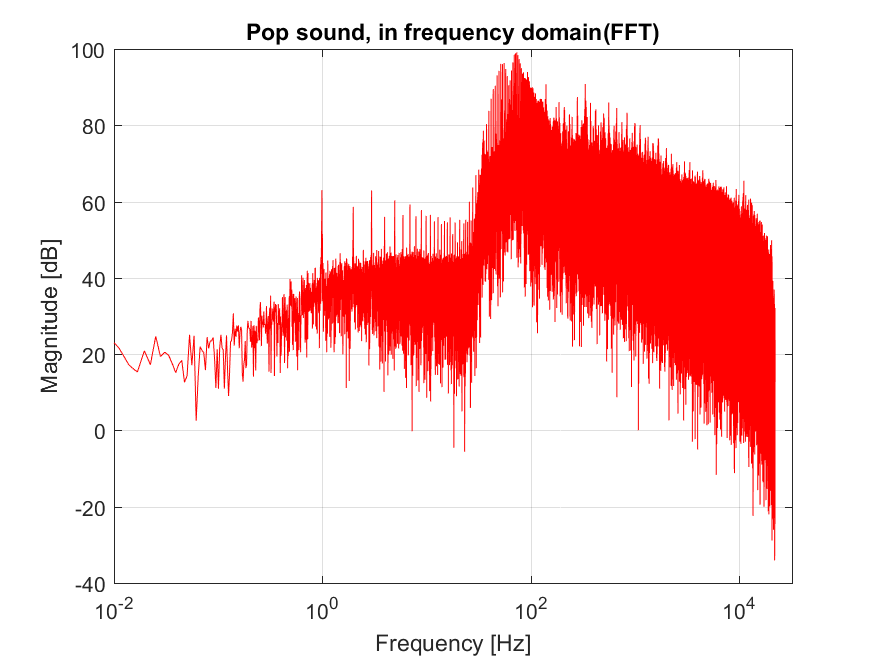
\includegraphics[width=0.45\linewidth]{code/Pop_figure2.png}}
	\subcaptionbox{Smoothed fft.\label{fig:pop_smooth}}
	{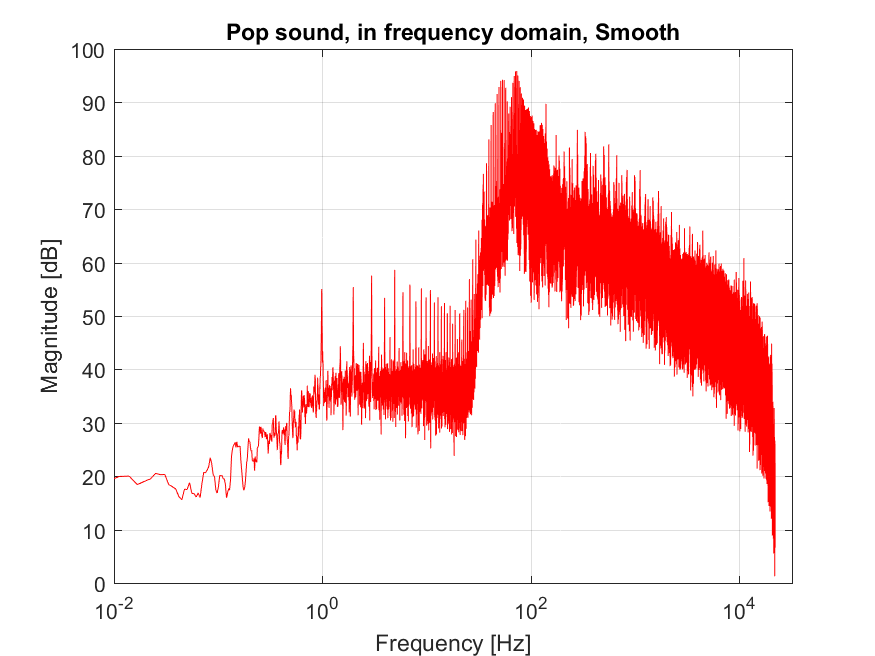
\includegraphics[width=0.45\linewidth]{code/Pop_figure3.png}}
	\subcaptionbox{fft of zero padded original.\label{fig:pop_zero}}
	{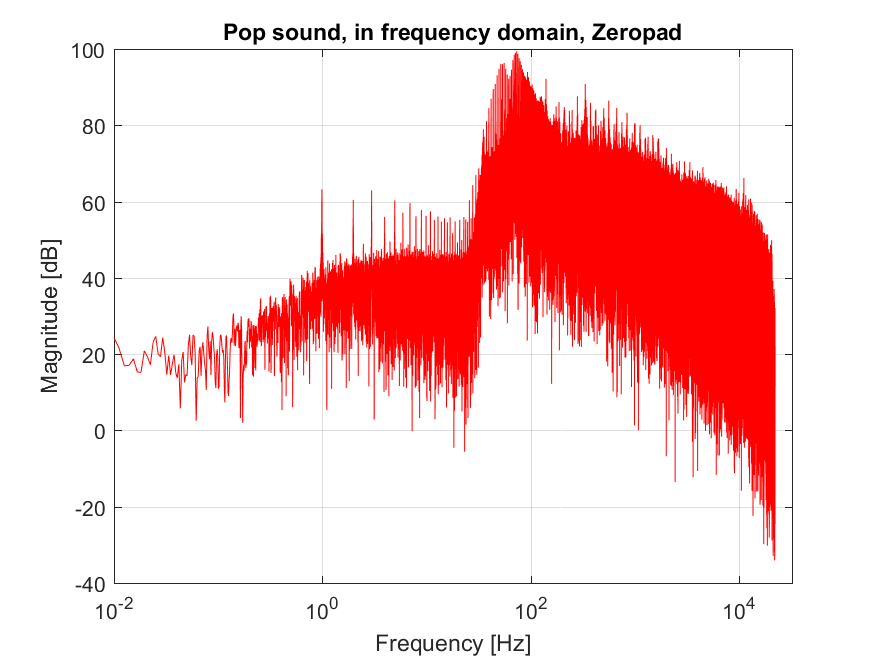
\includegraphics[width=0.45\linewidth]{code/Pop_figure4.png}}
	\subcaptionbox{fft of windowed original.\label{fig:pop_window}}
	{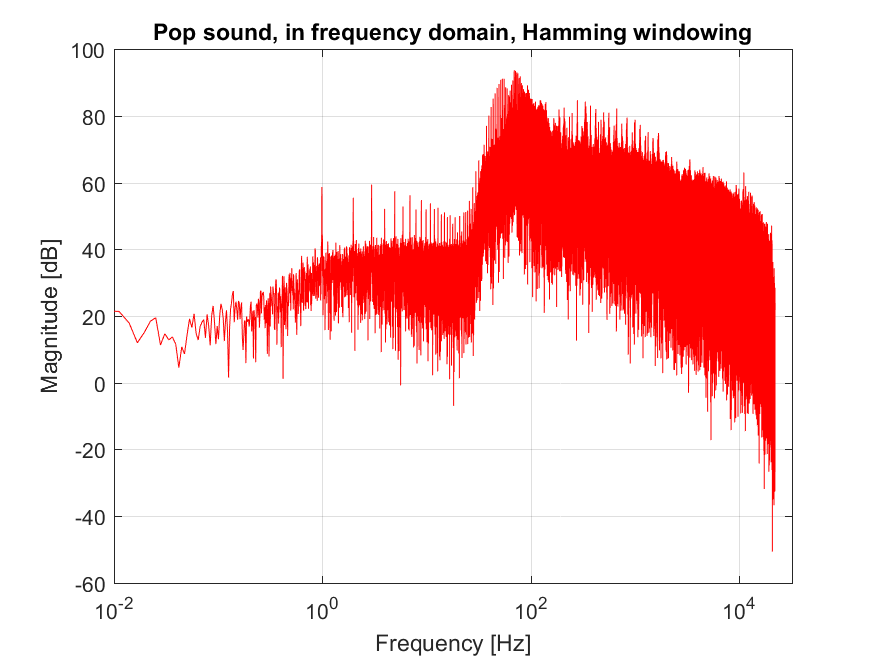
\includegraphics[width=0.45\linewidth]{code/Pop_figure5.png}}
	\caption{Analysis of the sound of Pop.}\label{fig:pop}
\end{figure}

\paragraph{Tekno}
Matador - The Enemy ft Felix Da Housecat (Original Mix)


The original signal from the song "The Enemy" is seen plotted in the timedomain in figure \ref{fig:techno_time}, while the fourier transformed signal is seen in figure \ref{fig:techno_freq}. The following has first applied some function and then is fourier transformed, the smooth function is seen on figure \ref{fig:techno_smooth}, the zeropadding is seen in figure \ref{fig:techno_zero} and the window function is seen in figure \ref{fig:techno_window}.

\begin{figure}[htb!]
	\centering
	\subcaptionbox{Time Domain.\label{fig:techno_time}}
	{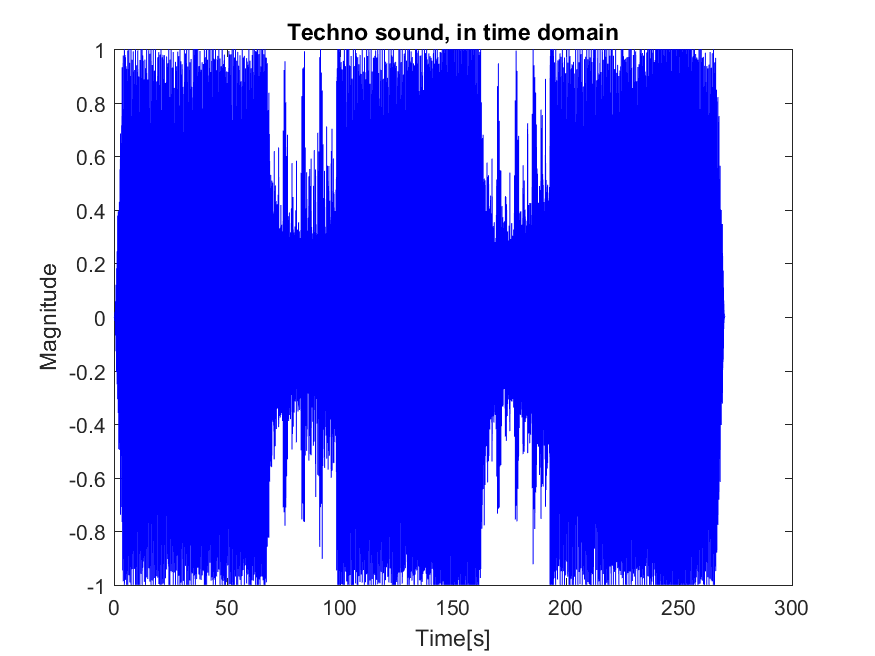
\includegraphics[width=0.45\linewidth]{code/Techno_figure1.png}}
	\subcaptionbox{Frequency Domain.\label{fig:techno_freq}}
	{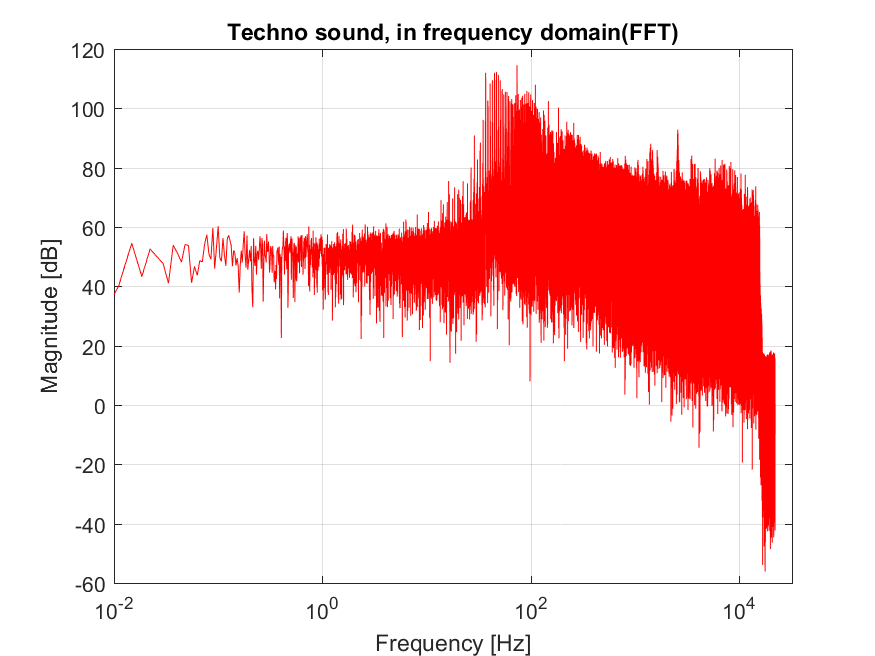
\includegraphics[width=0.45\linewidth]{code/Techno_figure2.png}}
	\subcaptionbox{Smoothed fft.\label{fig:techno_smooth}}
	{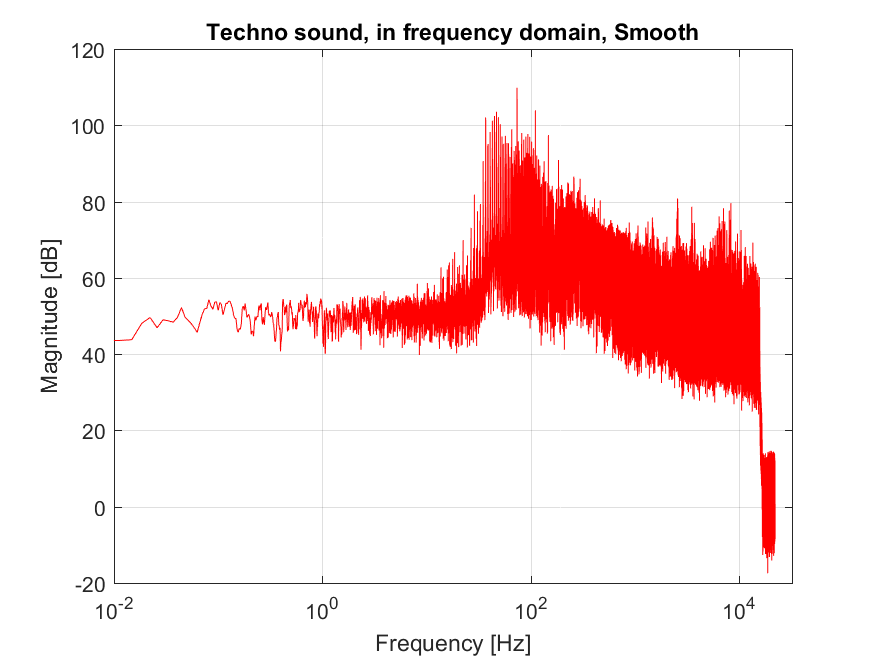
\includegraphics[width=0.45\linewidth]{code/Techno_figure3.png}}
	\subcaptionbox{fft of zero padded original.\label{fig:techno_zero}}
	{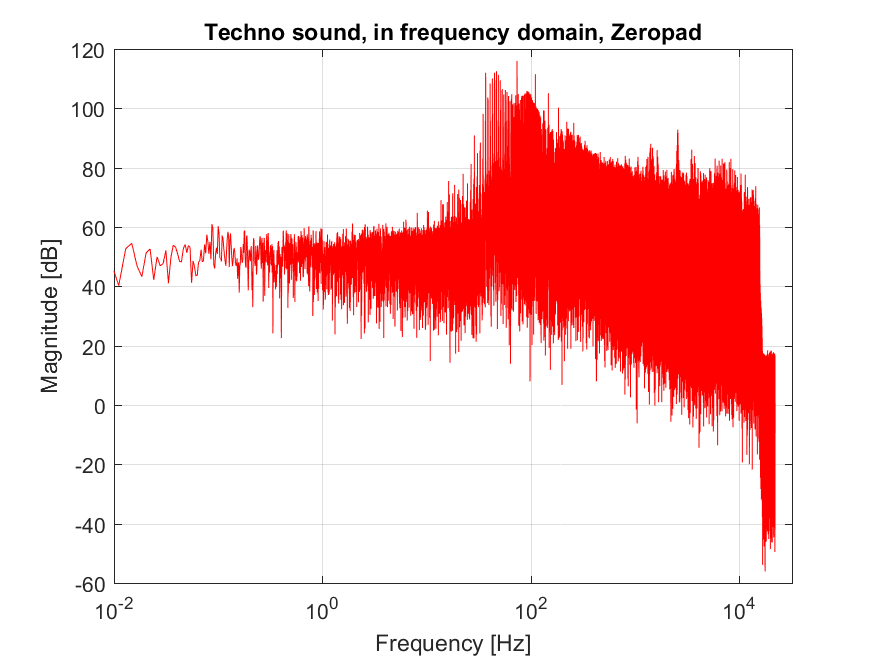
\includegraphics[width=0.45\linewidth]{code/Techno_figure4.png}}
	\subcaptionbox{fft of windowed original.\label{fig:techno_window}}
	{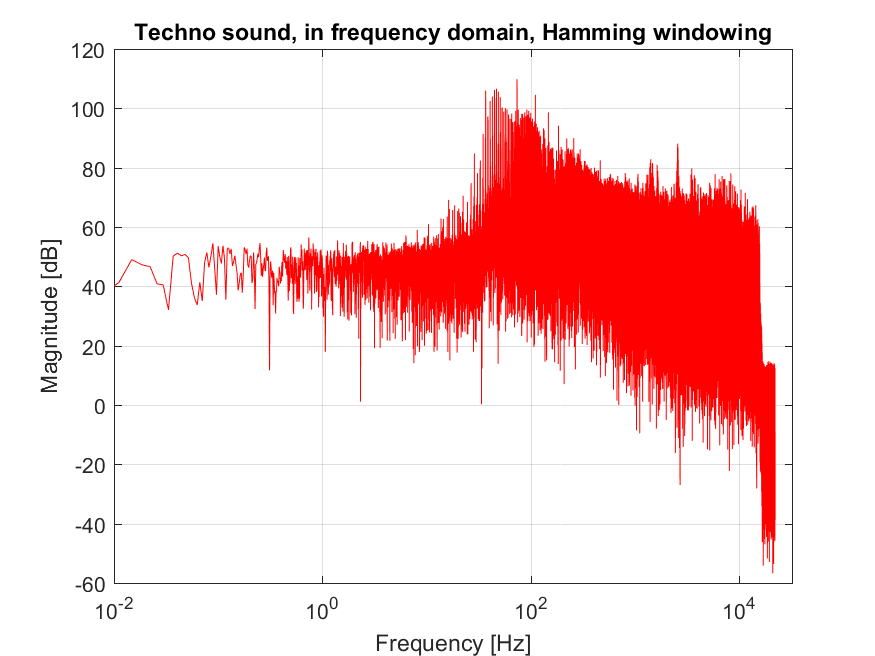
\includegraphics[width=0.45\linewidth]{code/Techno_figure5.png}}
	\caption{Analysis of the sound of Techno.}\label{fig:techno}
\end{figure}

\paragraph{Heavy Metal}

\paragraph{Klassisk}

\subsubsection{Conclusion}


\section{Energy} 
\Cref{tab:Energy} shows the energies in signals before and after the Fourier transform. It clearly shows that there is no loss of energy between the original signal and a Fourier transform, but when smoothing and windowing is applied there is a potential loss of energy.
While zero padding does not add or remove any energy from the signal.
\begin{table}[htb!]
	\centering
	\begin{tabularx}{\textwidth}{p{2cm} | X X X X X}
		& \rotatebox{90}{\textbf{Time Domain $\times\num{e4}$}}   & \rotatebox{90}{\textbf{Frequency Domain $\times\num{e4}$}} & \rotatebox{90}{\textbf{Smooth $\times\num{e3}$}}     & \rotatebox{90}{\textbf{Zero Padding $\times\num{e4}$}}  & \rotatebox{90}{\textbf{Windowing $\times\num{e4}$}} \\
		\hline
		Car Engine  & \num{3,07}	& \num{3,07}	& \num{0,686}  &	\num{3,07}  & \num{1,34}  \\
		
		Windmill	& \num{4,14}	& \num{4,14}	& \num{0,521} & \num{4,14} & \num{1,79} \\
		
		Breaking Wine Glass & \num{0,0115}	& \num{0,0115}	& \num{0,155}	& \num{0,0115}	& \num{0,000265} \\
		
		EKG & \num{2,05}	& \num{2,05}	& \num{0,626}	& \num{2,05}	& \num{0,729} \\
		
		Pop & & & & & \\
		
		Electronica & & & & & \\
		
		Heavy Metal & & & & & \\
		
		Klassisk & & & & & \\
	\end{tabularx}
	
	\caption{Energy of the different signals shown in \si{\joule}.}
	\label{tab:Energy}
\end{table}

Eksperimenter med udglatning, zero-padding og windowing 
\clearpage
\section{Energy} 
\Cref{tab:Energy} shows the energies in signals before and after the Fourier transform. It clearly shows that there is no loss of energy between the original signal and a Fourier transform, but when smoothing and windowing is applied there is a potential loss of energy.
Zero padding does not add or remove any energy from the signal, as it is equivalent to adding \SI{0}{\volt}DC to the signal.
\begin{table}[htb!]
	\centering
	\begin{tabularx}{\textwidth}{p{2cm} | X X X X X}
		& \rotatebox{90}{\textbf{Time Domain $\times\num{e4}$}}   & \rotatebox{90}{\textbf{Frequency Domain $\times\num{e4}$}} & \rotatebox{90}{\textbf{Smooth $\times\num{e3}$}}     & \rotatebox{90}{\textbf{Zero Padding $\times\num{e4}$}}  & \rotatebox{90}{\textbf{Windowing $\times\num{e4}$}} \\
		\hline
		Car Engine  & \num{3,07}	& \num{3,07}	& \num{0,686}  &	\num{3,07}  & \num{1,34}  \\
		
		Windmill	& \num{3,45}	& \num{3,45}	& \num{0,252} & \num{3,45} & \num{1,45} \\
		
		Breaking Wine Glass & \num{0,00666}	& \num{0,00666}	& \num{0,903}	& \num{0,00666}	& \num{0,000724} \\
		
		EKG & \num{0,960}	& \num{0,960}	& \num{0,731}	& \num{0,960}	& \num{0,369} \\
		
		Pop & \num{73,3}	& \num{73,3}	& \num{2,06}	& \num{73,3}	& \num{34,0} \\
		
		Techno & \num{101}	& \num{101}		& \num{1,56}	& \num{101}		& \num{37,2} \\
		
		Heavy Metal & \num{21,1} &	\num{21,1} & \num{1,48}	& \num{21,1}	& \num{9,07} \\
		
		Classical & \num{12,9}	& \num{12,9}	& \num{1,09}	& \num{12,9}	& \num{3,86} \\
	\end{tabularx}
	\caption{Energy of the different signals shown in \si{\joule}.}
	\label{tab:Energy}
\end{table}
\clearpage
<<<<<<< HEAD
\section{Frequency analysis}
\label{sec:analysis}
\subsection{Car engine}
\begin{figure}[htb]
	\centering
	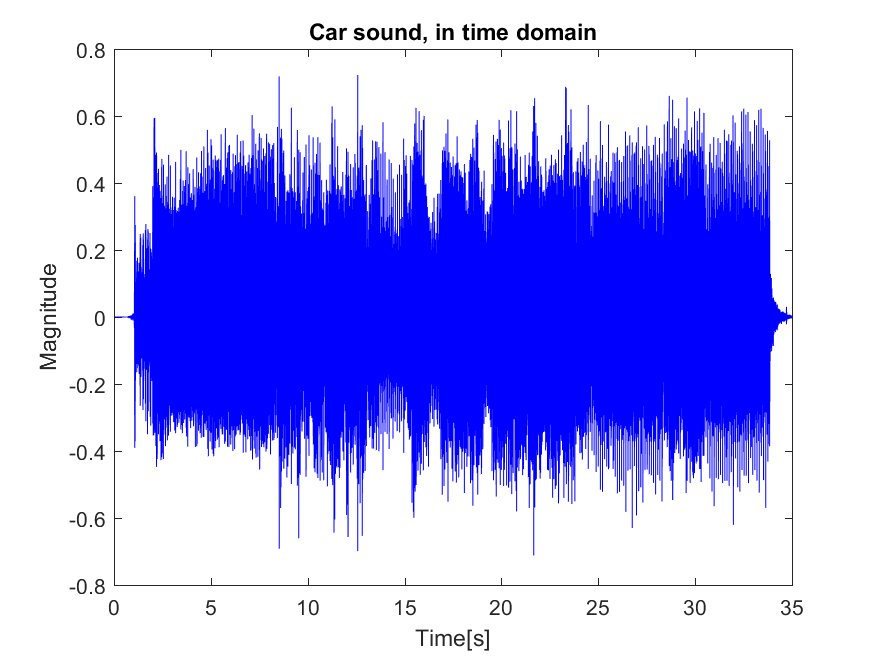
\includegraphics[width=.5\textwidth]{code/Car_figure1.png}
	\caption{The sound of a car shown in the Time Domain.}
	\label{fig:Car_figure1:1}
\end{figure}

\subsubsection{DFT}
\begin{figure}[htb]
	\centering
	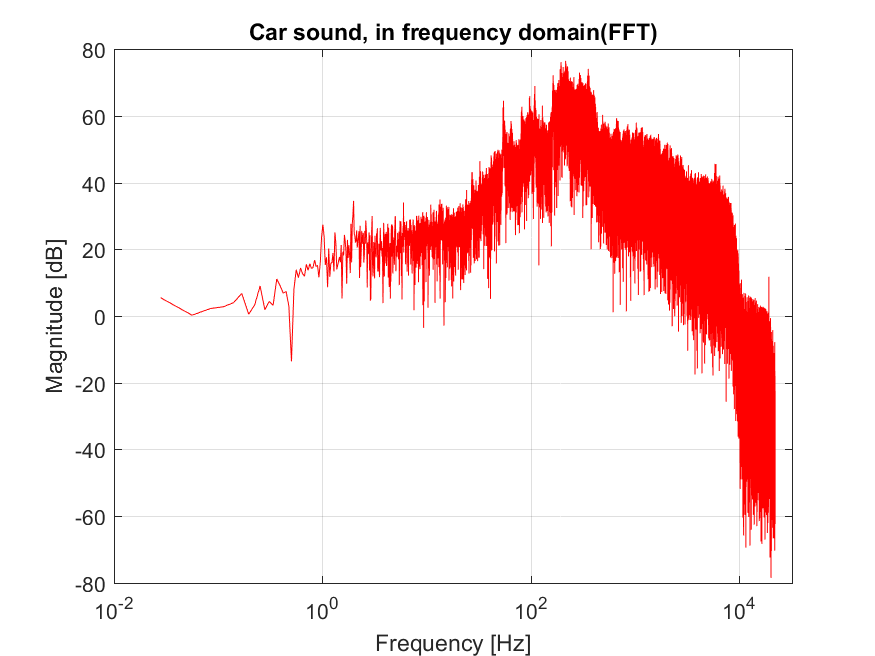
\includegraphics[width=.5\textwidth]{code/Car_figure2.png}
	\caption{The sound of a car shown in the Frequency Domain.}
	\label{fig:Car_figure2:2}
\end{figure}
=======

>>>>>>> 624490c0407af64f23ba273babf72d62fcadad27




<<<<<<< HEAD
\subsubsection{Analysis}



\subsubsection{Conclusion}

\subsection{Noise from a windmill}
\subsubsection{DFT}

\subsubsection{Analysis}

\subsubsection{Conclusion}

\subsection{EKG}
\subsubsection{DFT}

\subsubsection{Analysis}

\subsubsection{Conclusion}

\subsection{Breaking wine glass}
\subsubsection{DFT}

\subsubsection{Analysis}

\subsubsection{Conclusion}

\subsection{Music}
\subsubsection{DFT}

\subsubsection{Analysis}

\paragraph{Genre 1}

\paragraph{Genre 2}

\paragraph{Genre 3}

\paragraph{Genre 4}

\subsubsection{Conclusion}
=======

>>>>>>> 624490c0407af64f23ba273babf72d62fcadad27


\section{Energy} 
\Cref{tab:Energy} shows the energies in signals before and after the Fourier transform. It clearly shows that there is no loss of energy between the original signal and a Fourier transform, but when smoothing and windowing is applied there is a potential loss of energy.
While zero padding does not add or remove any energy from the signal.
\begin{table}[]
	\centering
	\begin{tabularx}{\textwidth}{p{2cm} | X X X X X}
		& \rotatebox{90}{\textbf{Time Domain $\times\num{e4}$}}   & \rotatebox{90}{\textbf{Frequency Domain $\times\num{e4}$}} & \rotatebox{90}{\textbf{Smooth $\times\num{e3}$}}     & \rotatebox{90}{\textbf{Zero Padding $\times\num{e4}$}}  & \rotatebox{90}{\textbf{Windowing $\times\num{e4}$}} \\
		\hline
		Windmill	& \num{4,14}	& \num{4,14}	& \num{0,521} & \num{4,14} & \num{1,79} \\

		Car Engine  & \num{3,07}	& \num{3,07}	& \num{0,686}  &	\num{3,07}  & \num{1,34}  \\

		Cheerleader & \num{13,4}	& \num{13,4}	& \num{1,29}	& \num{13,4}	& \num{7,39}  \\

		Roundtable Rival & \num{29,8}	& \num{29,8}	& \num{1,70}	& \num{29,8}	& \num{12,8}5  \\

		Micheal Jackson \newline Billie Jean & \num{16,3}	& \num{16,3}	& \num{1,73}	& \num{16,3}	& \num{6,86} \\

		Violin \newline Let It Go & \num{2,24}	& \num{2,24}	& \num{0,896}	& \num{2,24}	& \num{1,09}  \\

		Krystalglas knuses & \num{0,0115}	& \num{0,0115}	& \num{0,155}	& \num{0,0115}	& \num{0,000265} \\

		EKG & \num{2,05}	& \num{2,05}	& \num{0,626}	& \num{2,05}	& \num{0,729}
	\end{tabularx}
	
	\caption{Energy of the different signals shown in \si{\joule}.}
	\label{tab:Energy}
\end{table}

\section{Discussion}

Skalering --> Vi kan ikke bruge frekvenser højere end nyquits frekvens ?
Korrekte frekvensbins?

\section{Conclusion}

%\section{appendix}

\printbibliography

\end{document}
